\chapter{Wav-Manipulation und Analyse}

In diesem Kapitel wird anhand von Spektrogrammen, die mit Python und der Bibliothek \texttt{librosa} generiert wurden, die Analyse und Visualisierung der harmonischen und perkussiven Komponenten des Audiosignals demonstriert. Der Fokus liegt auf den Frequenzverteilungen und der Amplitudenhüllkurve.

\section{Spektralanalyse der Audiodatei}

Im Folgenden wird die Frequenzverteilung des Audiosignals vor und nach der Trennung in harmonische und perkussive Komponenten dargestellt. Diese Analyse ermöglicht es, die Struktur des Signals und die Unterschiede zwischen den beiden Komponenten zu visualisieren.	

\subsection{Spektrogramm der Originaldatei}

\begin{figure}
    \centering
    \includegraphics[width=0.8\textwidth]{AudioAnalysis.png}
    \caption{Spektrogramm der Original-Audiodatei vor der Trennung}
    \label{fig:audio_analysis}
\end{figure}

Abbildung \ref{fig:audio_analysis} zeigt das Spektrogramm des ungetrennten Audiosignals. Die Farbskala stellt die Amplituden der Frequenzanteile dar, wobei hellere Farben höhere Amplituden repräsentieren. Dieses Spektrogramm stellt das gesamte Frequenzspektrum dar, das sowohl harmonische als auch perkussive Elemente enthält.

\subsection{Spektrogramm der harmonischen Komponente}

\begin{figure}
    \centering
    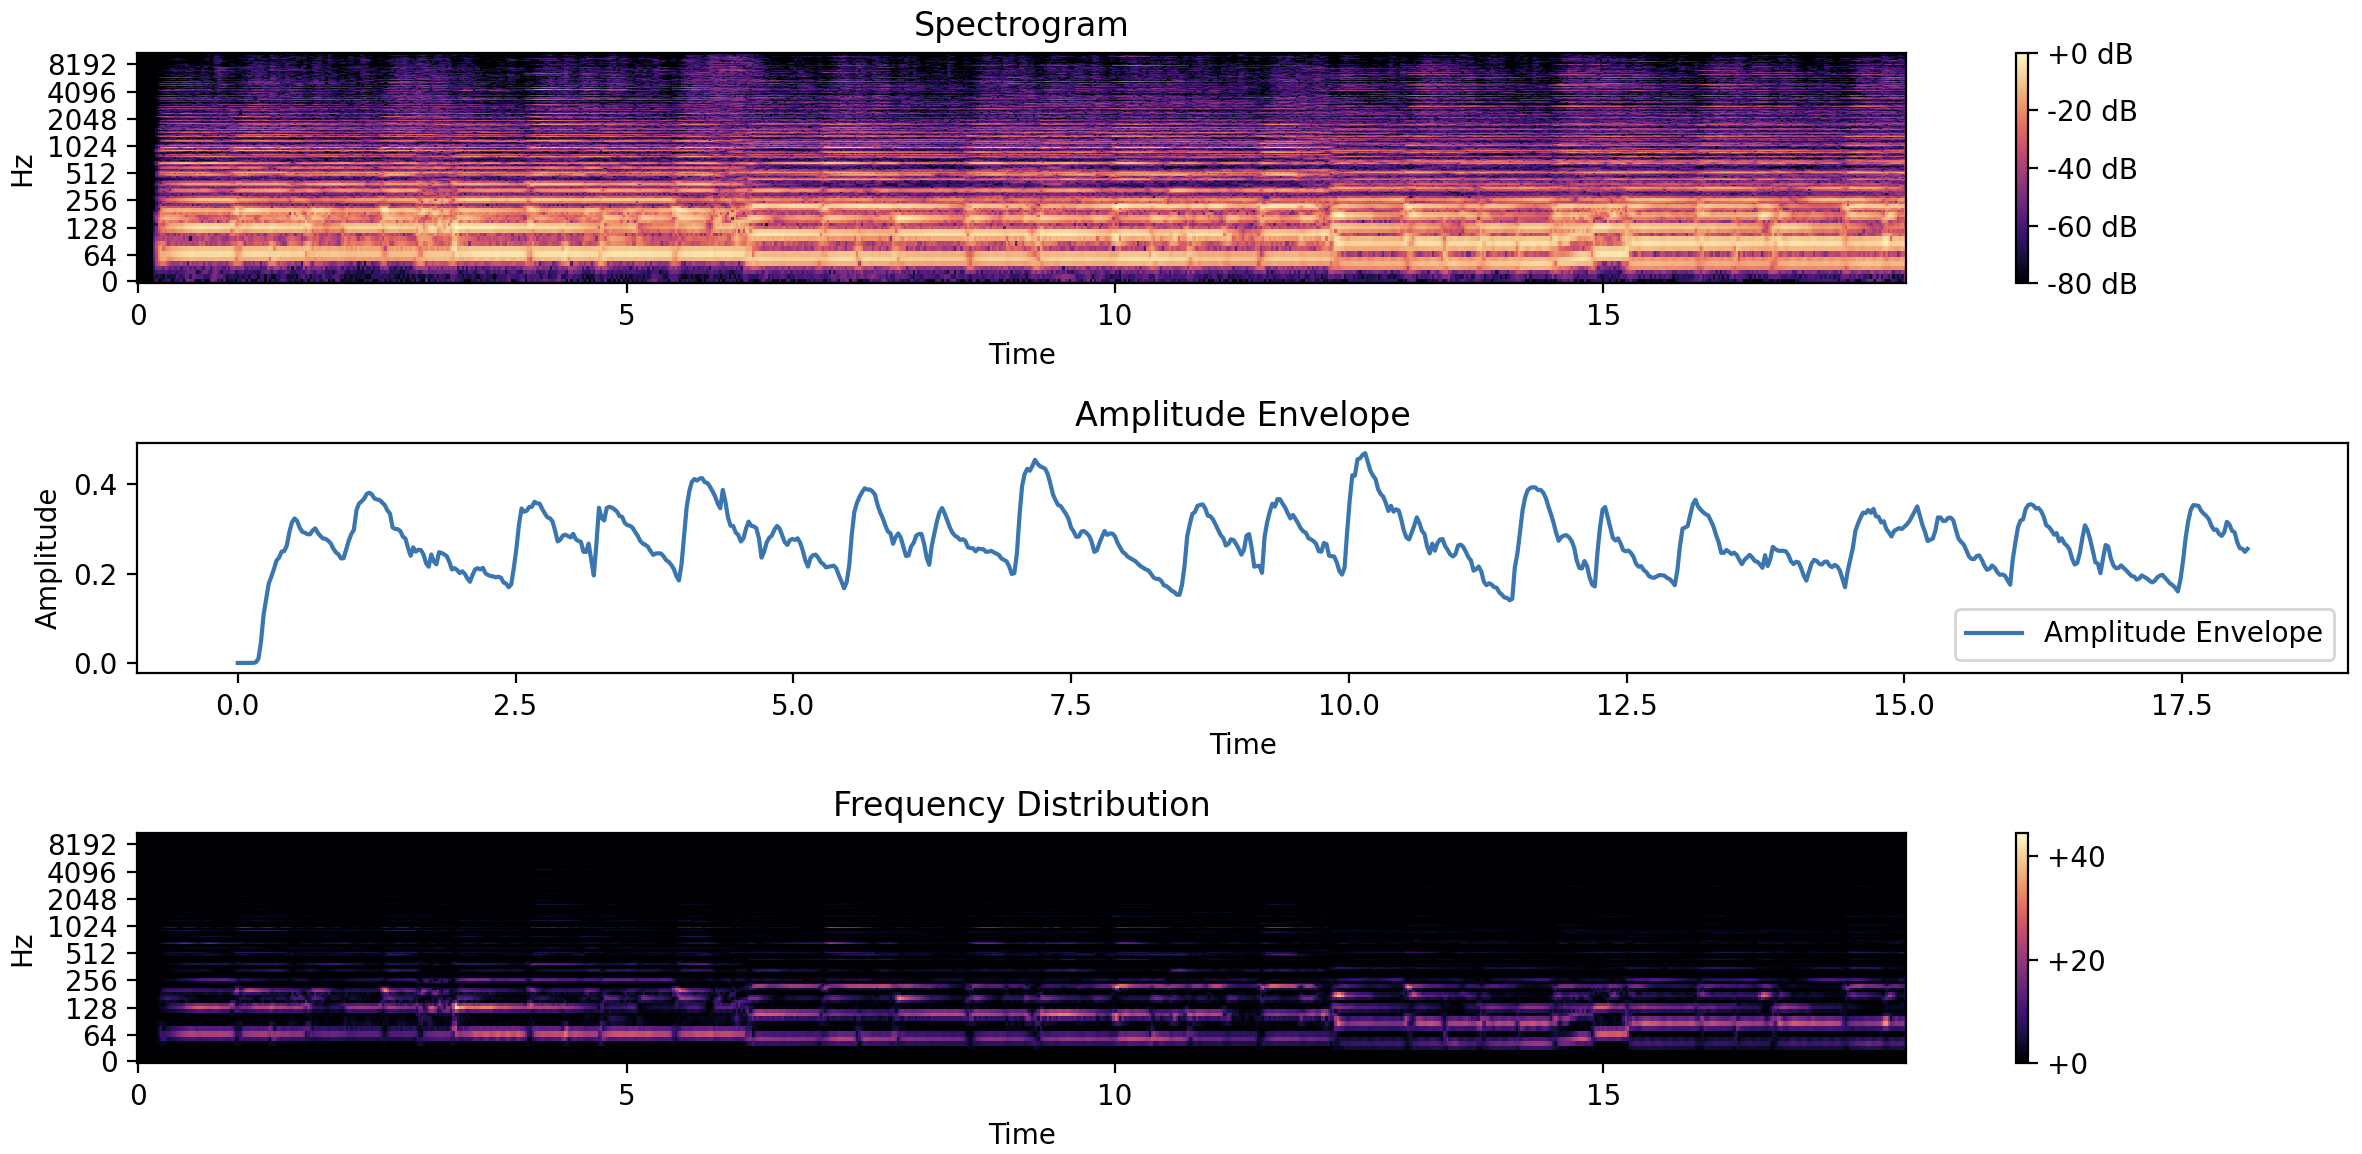
\includegraphics[width=0.8\textwidth]{HarmonicAnalysis.png}
    \caption{Spektrogramm der harmonischen Komponente}
    \label{fig:harmonic_analysis}
\end{figure}

Abbildung \ref{fig:harmonic_analysis} zeigt das Spektrogramm der harmonischen Komponente nach der Trennung. Die harmonischen Komponenten des Signals sind Frequenzen, die stabil und langanhaltend sind, was typisch für melodische oder gesangliche Elemente ist. Man sieht eine gleichmäßigere Verteilung im Frequenzbereich mit weniger plötzlichen Amplitudenänderungen.

\subsection{Spektrogramm der perkussiven Komponente}

\begin{figure}
    \centering
    \includegraphics[width=0.8\textwidth]{PercussiveAnalysis.png}
    \caption{Spektrogramm der perkussiven Komponente}
    \label{fig:percussive_analysis}
\end{figure}

Abbildung \ref{fig:percussive_analysis} zeigt das Spektrogramm der perkussiven Komponente. Die perkussiven Elemente zeigen eine charakteristische Struktur, da sie Frequenzen darstellen, die plötzliche Änderungen aufweisen, typischerweise durch kurze, abrupte Schläge oder rhythmische Akzente gekennzeichnet.

\section{Interpretation der Ergebnisse}

Durch die Trennung der Audiodatei in harmonische und perkussive Komponenten wird die Spektralanalyse differenziert. Harmonische Spektren zeigen konstante, langanhaltende Frequenzen, während perkussive Spektren kurze, intensive Peaks aufweisen. Dies erlaubt eine gezielte Analyse und Bearbeitung der musikalischen Elemente, die für verschiedene Audioverarbeitungsaufgaben wie die Musikproduktion, Remixing oder Audio-Restaurierung wertvoll ist.
